% Qualitative window behavior; no UI elements or simulated measurements.
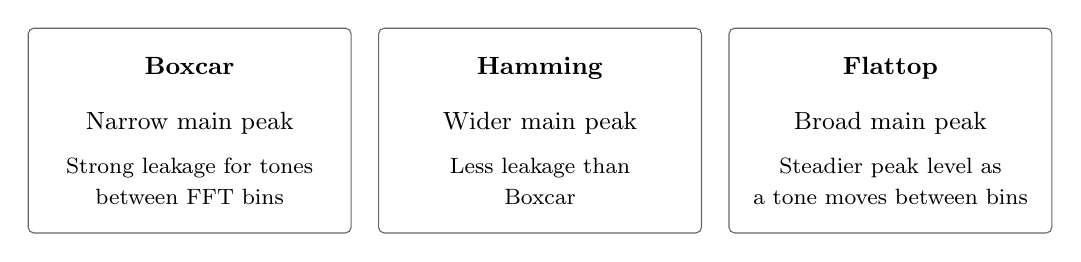
\begin{tikzpicture}[x=1cm,y=1cm,font=\small,
    card/.style={draw=black!60,rounded corners=2pt,minimum width=4.1cm,
      minimum height=2.6cm,align=center}]
  \node[card] at (2.05,0) {\textbf{Boxcar}\\[9pt]
    Narrow main peak\\[5pt]\footnotesize Strong leakage for tones\\
    \footnotesize between FFT bins};
  \node[card] at (6.5,0) {\textbf{Hamming}\\[9pt]
    Wider main peak\\[5pt]\footnotesize Less leakage than\\
    \footnotesize Boxcar};
  \node[card] at (10.95,0) {\textbf{Flattop}\\[9pt]
    Broad main peak\\[5pt]\footnotesize Steadier peak level as\\
    \footnotesize a tone moves between bins};
\end{tikzpicture}
